\documentclass{article}

\usepackage[brazil]{babel}
\usepackage[utf8]{inputenc}
\usepackage{amsmath}
\usepackage{amsfonts}

\usepackage[section]{placeins}

\usepackage{graphicx}

\usepackage{color} %red, green, blue, yellow, cyan, magenta, black, white
\definecolor{mygreen}{RGB}{28,172,0} % color values Red, Green, Blue
\definecolor{mylilas}{RGB}{170,55,241}

\begin{document}

\begin{flushleft}
\textbf{FUNDAÇÃO GETÚLIO VARGAS} \\

\textbf{Escola de Pós-Graduação em Economia}

\textbf{Teoria Macroeconômica III - Lista 02}

Professor: Ricardo de Oliveira Cavalcanti

Monitora: Kátia Aiko Nishiyama Alves

Alunos: Samuel Barbosa e Gustavo Bulhões
\end{flushleft}

\section*{Exercício 01}
Considere a função $f(x) = x^3 \exp(-x^2)$. Vamos encontrar o máximo global desta função
aplicando o método da biseção (i) e o método de Newton-Rhapson (ii) para econtrar 
as raízes da primeira derivada de $f$, dada por $$f'(x) = x^2 (3-2x^2) e^{-x^2}.$$

\subsection*{Item (i)}

Neste método iniciamos com um intervalo $[a,b]$
tal que $f(a) f(b) < 0$ Se $f$ é contínua, pelo Teorema do Valor Intermediário 
existe um $x^* \in (a,b)$ tal que $f(x^*) = 0$.

Para encontrá-lo, dividimos o intervalo no ponto médio do intervalo

$$ c = \frac{a + b}{2}$$

e avaliamos $f(a) f(c)$. Se $f(a) f(c)$ é negativo, então o 
Teorema do Valor Intermediário garante a existência de uma raiz no intervalo
$(a,c)$. Se por outro lado $f(a) f(c)$ é positivo, então a raiz pertence ao intervalo
$[c,b)$. Iteramos este procedimento até obter um intervalo suficientemente pequeno.

Antes de aplicar o método, vamos delimitar o intervalo inicial a partir do gráfico de $f$:

\begin{figure}[!h]
  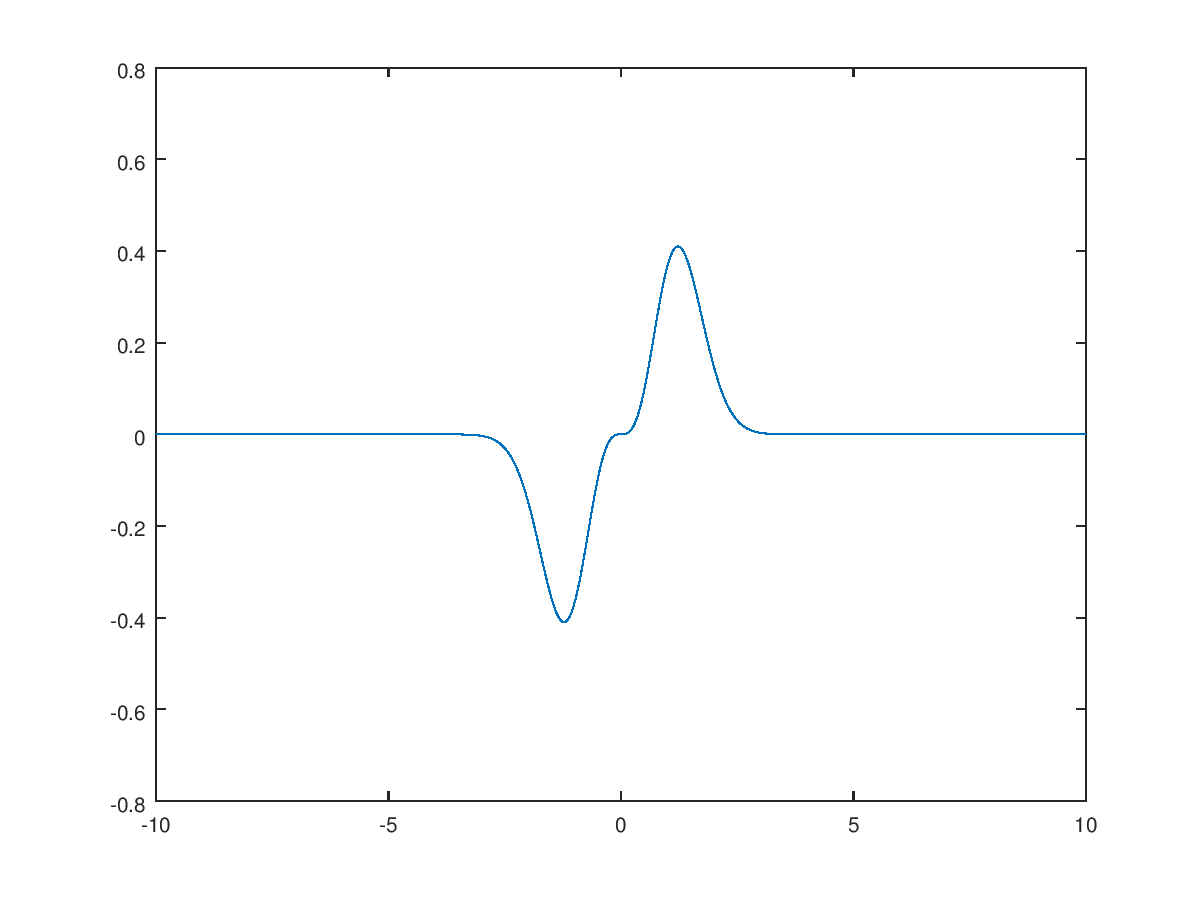
\includegraphics[scale=0.6]{ex1/ex1_1.png}
\end{figure}

\newpage

Observe que $f$ tem vários pontos críticos. É fácil identificar graficamente que 
o ponto de máximo da função está entre 0 e 5. Como 0 é ponto de inflexão, contudo,
vamos retirá-lo do intervalo inicial, que delimitaremos em $[0.1, 5]$.

Aplicando o método no intervalo especificado, obtemos o ponto de máximo global da 
função $f$ em $x = 1.2247$.

\subsection*{Item (ii)}

No método de Newton-Rhapson, definimos um valor inicial de $x_0$ dentro de
um intervalo $[a,b]$ e calculamos a reta tangente a $f$ neste ponto. 
Temos então uma aproximação linear de $f$ em torno do ponto $x_0$. 
Escolhemos a raiz desta função linear como uma melhor estimativa da raiz 
da função original $f$. Iteramos este procedimento até obter
convergência da estimativa. Se em uma dada iteração a estimativa da raiz 
assumir valor fora do intervalo $[a,b]$, sorteamos um novo $x_0$ 
dentro do intervalo e reiniciamos o algoritmo.

Aplicando este método no intervalo $[0.1, 5]$ obtemos a mesma solução do item anterior.

\subsection*{Item (iii)}

A tabela a seguir traz uma comparação dos métodos em termos de número de iterações e
tempo decorrido. Como o método de Newton-Rhapson incorpora um componente aleatório
(eventual necessidade de sortear novos valores iniciais), reportamos a média de iterações
e do tempo decorrido em 10.000 aplicações do algoritmo. \\

\begin{tabular}{ccc}
 Método   		& Iterações & Tempo decorrido (s) \\ \hline
 Bisseção 		& 	 54     &       0.0050        \\
 Newton-Rhapson & 	 57     &       0.0046  	  \\
\end{tabular} \\ \\

Portanto, dada a função objetivo e o intervalo utilizado, concluimos que os 
métodos têm desempenho equivalente.

\section*{Exercício 02}

Neste exercício aplicamos a generalização do método de Newton-Rhapson para o caso multivariado.
Em particular vamos encontrar o ponto de máximo da função

$$ f(x,y) = \frac{4}{(x-1)^2 + 4y^2 + 1}.$$ \\

Observando o gráfico de $f$ vemos que podemos restringir nossa busca a $[-5,5] \times [-5,5]$,
com $(0,0)$ sendo um bom chute inicial. 

\begin{figure}[!h]
  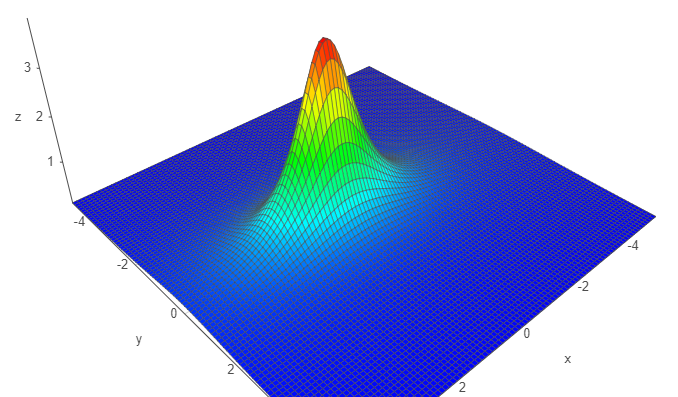
\includegraphics[scale=0.6]{ex2/ex2_1.png}
\end{figure}

\newpage

Aplicando o algoritmo, obtemos: \\ \\

\begin{tabular}{cccc}
	\hline Iteração & x & y & f(x,y) \\ \hline
	1  &  0.00000 & 0 & 2.00000 \\
	2  & -1.00000 & 0 & 0.80000 \\
	3  & -1.90909 & 0 & 0.42271 \\
	4  & -3.03783 & 0 & 0.23116 \\
	5  & -4.49614 & 0 & 0.12817 \\
	6  &  1.34663 & 0 & 3.57093 \\
	7  &  0.73950 & 0 & 3.74581 \\
	8  &  1.08879 & 0 & 3.96872 \\
	9  &  0.99713 & 0 & 3.99997 \\
	10 &  1.00000 & 0 & 4.00000 \\
	11 &  1.00000 & 0 & 4.00000  \\ \hline
\end{tabular} \\ \\ 

com $x^* = 1$, $y^*=0$, e $f(x^*,y^*)=4$.

\end{document}

